\documentclass{article}
\usepackage{amsmath}
\usepackage{amssymb}
\usepackage{graphicx}

\begin{document}

\section{Basic SGD}
\subsection{Constant step size}
\begin{figure}[h!]
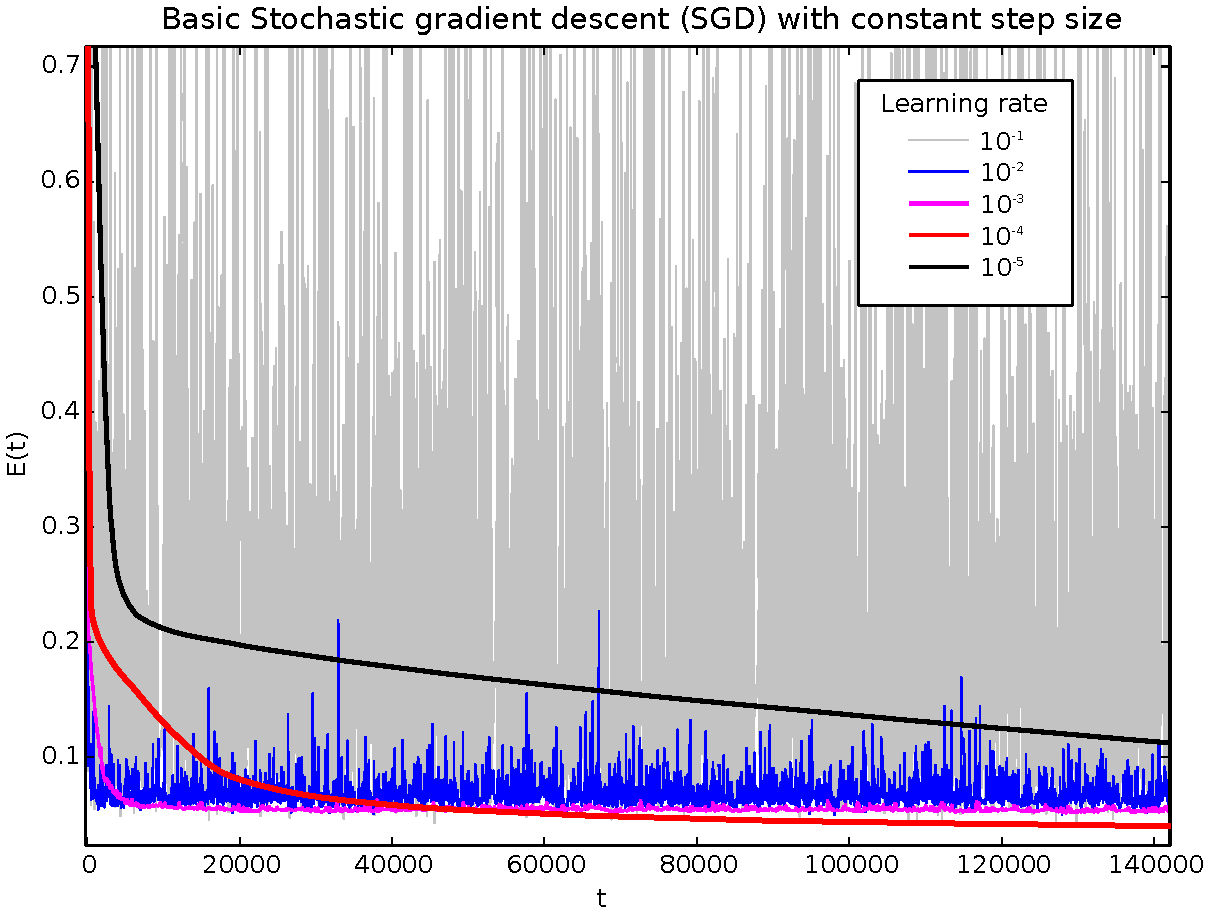
\includegraphics[width=\textwidth]{SG_constant_step.pdf}
\caption{(MNIST objective on train data $n=60000$.)}
\end{figure}
Problem : Does not converge exactly .
\begin{itemize}
\item large step $\Rightarrow$ fast but doesn't converge up to some minimal error $\epsilon$ (fast but rough). \item Small step $\Rightarrow$ $\epsilon$ decreases but longer convergence (accurate but slow).
\end{itemize}
Trade-off has to be made between accuracy and convergence speed, through the fixed step size parameter $\eta$.

\subsection{Decreasing step size}

Let $\eta(t) = \frac{1}{\lambda t}$. $\eta$ is no more a parameter.

\begin{figure}[h!]
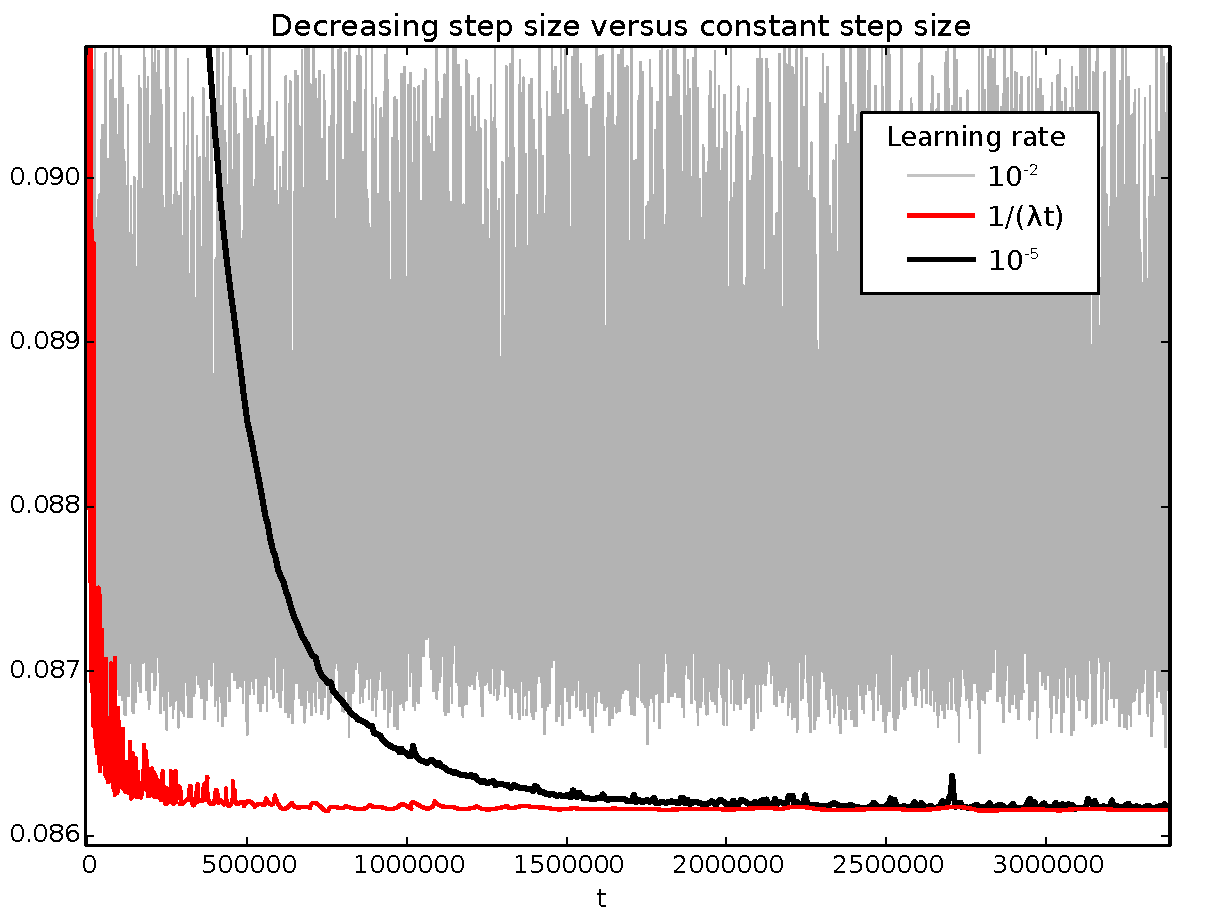
\includegraphics[width=\textwidth]{SG_decreasing_step.pdf}
\caption{(MNIST objective on train data $n=60000$.)}
\end{figure}

\end{document}